%coding:utf-8

%----------------------------------------
%FOSAPHY, a LaTeX-Code for a summary of optics
%Copyright (C) 2014, Mario Felder, Michael Fallegger

%This program is free software; you can redistribute it and/or
%modify it under the terms of the GNU General Public License
%as published by the Free Software Foundation; either version 2
%of the License, or (at your option) any later version.

%This program is distributed in the hope that it will be useful,
%but WITHOUT ANY WARRANTY; without even the implied warranty of
%MERCHANTABILITY or FITNESS FOR A PARTICULAR PURPOSE.  See the
%GNU General Public License for more details.
%----------------------------------------

\documentclass[a5paper,10pt,fleqn]{book}

\usepackage{layout}

\title{Formelsammlung Optik}

\author{Mario Felder\\Michi Fallegger}
\date{\today}

%\catcode `\*=\active
%\def *{\cdot}

\begin{document}

\maketitle
\thispagestyle{empty}
\cleardoublepage
\pagenumbering{Roman}
\tableofcontents

%coding:utf-8

%----------------------------------------
%FOSAPHY, a LaTeX-Code for a summary of optics
%Copyright (C) 2014, Mario Felder, Michael Fallegger

%This program is free software; you can redistribute it and/or
%modify it under the terms of the GNU General Public License
%as published by the Free Software Foundation; either version 2
%of the License, or (at your option) any later version.

%This program is distributed in the hope that it will be useful,
%but WITHOUT ANY WARRANTY; without even the implied warranty of
%MERCHANTABILITY or FITNESS FOR A PARTICULAR PURPOSE.  See the
%GNU General Public License for more details.
%----------------------------------------

	\setcounter{page}{1}
    \pagenumbering{arabic}
%coding:utf-8

%----------------------------------------
%FOSAPHY, a LaTeX-Code for a summary of optics
%Copyright (C) 2014, Mario Felder, Michael Fallegger

%This program is free software; you can redistribute it and/or
%modify it under the terms of the GNU General Public License
%as published by the Free Software Foundation; either version 2
%of the License, or (at your option) any later version.

%This program is distributed in the hope that it will be useful,
%but WITHOUT ANY WARRANTY; without even the implied warranty of
%MERCHANTABILITY or FITNESS FOR A PARTICULAR PURPOSE.  See the
%GNU General Public License for more details.
%----------------------------------------

\chapter{Strahlen Optik}

\section{Einleitung}
\begin{itemize}
	\item Einfallswinkel = Ausfallswinkel 
	\item Licht breitet sich von einem Punkt A zu einem Punkt B so aus, dass die Laufzeit minimal wird. \\
\end{itemize}
\
\section{Konstanten}
\[
\boxed{\begin{aligned}	
		&\text{Lichtgeschwindigkeit} \\
		&c = 299'792'458\text{ m/s}\\
	\end{aligned}}	\]
\\
\\
\section{Brechung und Brechungsindex n}
Brechungsindex: 
\[
	n= \frac{c}{c_{mat}}
\]
Brechungsgesetz von Snellius: 
\[
	n_A \cdot \sin \theta_A = n_B\cdot \sin \theta_B
\]

\begin{footnotesize}
	Der \textbf{Winkel} bezüglich der Grenzfläche-Lots.
\end{footnotesize}
\\
\\
\section{Strahlenverschiebung}
\[
	\Delta x = d \cdot \frac{ \sin (\theta_a -\theta_b ^`)}{\cos \theta_b ^`}
\]
\begin{center}
	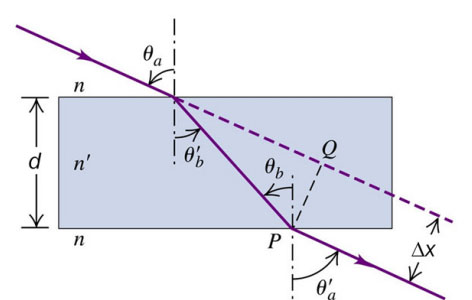
\includegraphics[scale = 0.3]{../fig/strahlenverschiebung.jpg}
\end{center}
\

\section{Totalreflexion}
Totalreflexion tritt auf, wenn der Grenzwinkel $\theta_krit$ überschritten wird.
\[
	\sin \theta_{krit} = \frac{n_B}{n_A}
\]
Totalreflexion Prisma:
\[
	\sin\frac{\alpha+\delta}{2} = n\cdot \sin \frac{\alpha}{2}
\]
\begin{center}
	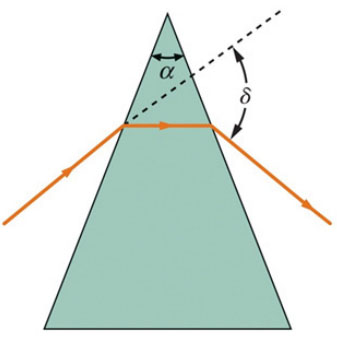
\includegraphics[scale = 0.2]{../fig/tr_prisma.jpg}
\end{center}
\
\section{Linsen}
\textbf{Sammellinsen, Konvexlinsen:} 
Dieser Linsentyp hat eine positive d.h. reelle Brennweite
\\
\textbf{Zerstreulinsen, Konkavlinsen:} 
Dieser Linsentyp hat eine negative, d.h. virtuelle Brennweite f

\subsection{Strahlkonstruktion bei dünnen Linsen}
Linsengleichung:
\[
	\frac{1}{f} = \frac{1}{g} + \frac{1}{b} \\
	\Rightarrow \\
	b=\frac{f \cdot g}{g -f} \\ \\
\]
\[
	\frac{B}{G} =\frac{b}{g}
\]
\begin{center}
	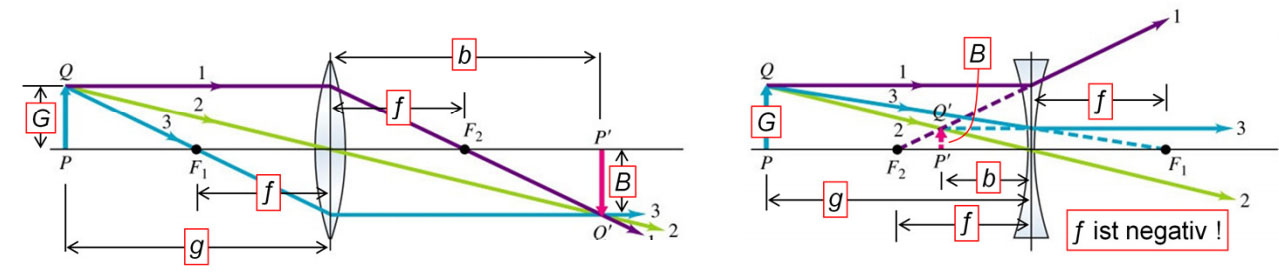
\includegraphics[scale = 0.25]{../fig/strahlkonstruktion.jpg}
\end{center}

\subsection{Vergrösserung}
Vergrösserung:
\[
	M=\frac{\theta^`}{\theta}= \frac{g_{NP}}{f} \approx \frac{25cm}{f}
\]
\begin{center}
	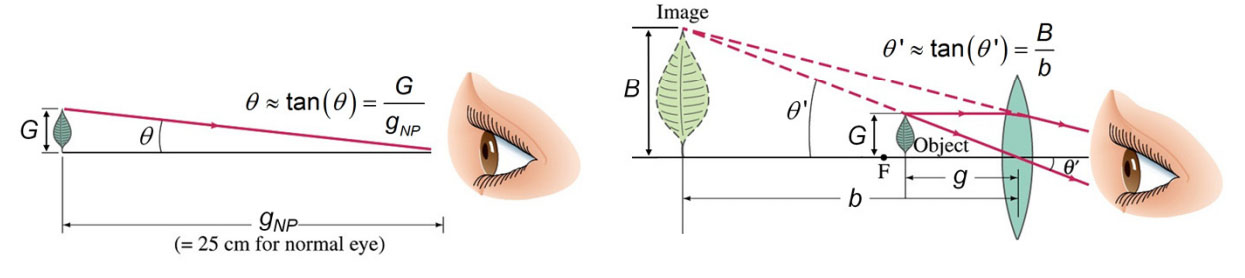
\includegraphics[scale = 0.25]{../fig/vergroesserung.jpg}
\end{center}

\subsection{Optische Instrumente: Mikroskop}
Vergrösserung eines Mikroskops:
\[
	M=m_1 \cdot m_2 = \frac{L\cdot g_{NP}}{f_0 \cdot f_e}
\]
\begin{center}
	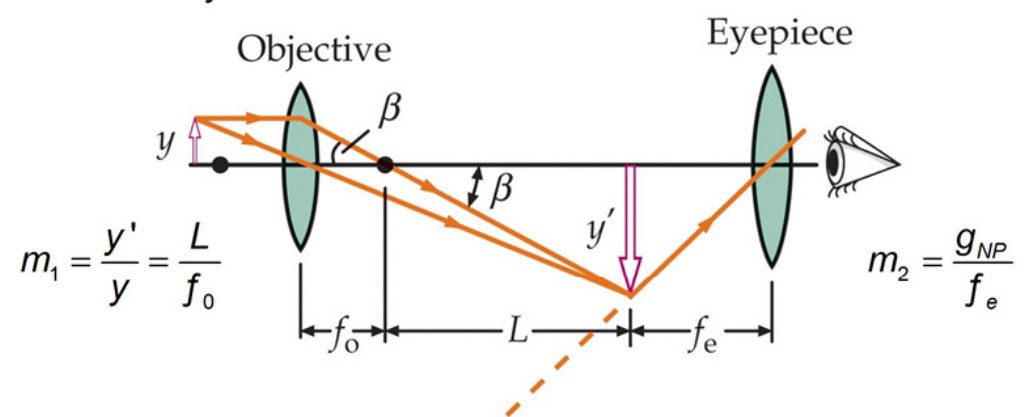
\includegraphics[scale = 0.2]{../fig/mikroskop.jpg}
\end{center}



%coding:utf-8

%----------------------------------------
%FOSAPHY, a LaTeX-Code for a summary of optics
%Copyright (C) 2014, Mario Felder, Michael Fallegger

%This program is free software; you can redistribute it and/or
%modify it under the terms of the GNU General Public License
%as published by the Free Software Foundation; either version 2
%of the License, or (at your option) any later version.

%This program is distributed in the hope that it will be useful,
%but WITHOUT ANY WARRANTY; without even the implied warranty of
%MERCHANTABILITY or FITNESS FOR A PARTICULAR PURPOSE.  See the
%GNU General Public License for more details.
%----------------------------------------

\chapter{Wellen Optik}
\section{Konstanten}
\[
\boxed{\begin{aligned}	
		&\varepsilon_0 = 8.85\cdot 10^{-12} As/Vm\\
		&\mu_0 = 4\pi \cdot 10^{-7} Vs/Am\\
		&n_{Wasser} = 1.3 \\
		&n_{Glas} = 1.5 \\
	\end{aligned}}	\]
\\
\section{Grundformeln}
Wellengeschwindigkeit:
\[
	v=\sqrt{\frac{F_S}{\mu}}
\]
\begin{footnotesize}
	$\mu$: Längenmasse
\end{footnotesize}
\\
\\
Harmonische Welle:
\[
	\lambda \cdot f = v
\]
Wellenzahl:
\[
	k=\frac{2\pi}{\lambda}=\frac{\omega}{v}
\]
\\
\section{EM Welle in einem transparenten Material}
Der Brechungsindex n beschreibt wie sich die Welle in einm transparenten Material fortbewegt.
\[
	c_0 \Rightarrow c=  \frac{c_0}{n} \\
	\lambda_0 \Rightarrow \lambda=  \frac{\lambda_0}{n} \\
	f \Rightarrow  konstant\\
\]
\\
\section{Dopplereffekt (Optik)}
Da eine EM Welle kein Medium braucht für die Fortbewegung, ist beim EM Dopplereffekt nur die relative Geschwindigkeit v zwischen Sender und Empfänger relevant.
\[
	f^`=f\cdot\sqrt{\frac{c-v}{c+v}}
\]
\\
\begin{footnotesize}
	v ist positiv bei Entfernung \\
	v ist negativ bei Annäherung \\
\end{footnotesize}
\\
\section{Reale Welle und komplexe Darstellung}	
Die komplexe Darstellung des E-Feld wird gewählt, weil die Berechnungen oft einfacher sind, insbesondere bei der Superposition (Additon) von Feldern und der Berechnung der Leistung.
\[
	E(x,t)=E_0\cdot e^{i(kx-\omega t +\phi_0)}
\]
\\
\section{Vergleich des E-Felds an zwei Punkten}
Positionsvergleich:
\[
	E(x+\Delta x,t)=E(x,t)\cdot e^{ik \Delta x}	
\]
Zeitvergleich:
\[
	E(x,t+\Delta t)=E(x,t)\cdot e^{-ik \Delta t} 
\]
Phasenverschiebung:
\[
	E(x_1,t_1)= E_0\cdot e^{i(kx_1-\omega t_1+\phi_0)}=E_0  \cdot e^{i\phi_1}
\]
\[
	E(x_2,t_2)= E_0\cdot e^{i(kx_2-\omega t_2+\phi_0)}=E(x_1,t_1)  \cdot e^{i\Delta \phi_1}
\]
\\
\section{Intensität einer EM Welle}
\[
	I=\frac{Leistung}{Fläche}=\frac{P}{A}=\frac{1}{2}\cdot nc_0\varepsilon_e |E_0|^2 
\]
\\
\[
	B_0\cdot e^{i(kx-\omega t)}\cdot (-i\omega) = 	
	E_0\cdot e^{i(kx-\omega t)}\cdot (ik)
\]
\[
	B_0=E \frac{k}{\omega}=E\frac{1}{c}
\]
\\
\begin{footnotesize}
	$c_0$:	Lichtgeschwindigkeit im Vakuum \\
	$n$:	Brechungsindex\\
	$\varepsilon_0$:	Dielektrizitätskonstante
\end{footnotesize}
\\
\section{Interferenz}
\begin{itemize}
	\item Konstruktive Interferenz: $\Delta\varphi=0$
	\item Destruktive Interferenz:  $\Delta\varphi=\pi$\\
\end{itemize}
Für Interferenzen zu addieren werden sie zuerst in das E-Feld zurück gerechnet.
\\
\\
Zeigerdiagramm:
\[
	E_{tot}(x,t)=E_{1,0}\cdot e^{i\phi_1}+E_{2,0}\cdot e^{i\phi_2}= (E_{1,0}+E_{2,0}\cdot e^{i\Delta\phi})\cdot e^{i(kx-\omega t)}
\]
\[
	I_{tot}= \frac{1}{2}nc_0\varepsilon_0|E_{tot}|^2 =
	\frac{1}{2}nc_0\varepsilon_0|E_{1,0}+E_{2,0}\cdot e^{i\Delta \phi}|^2
\]
Phasenverschiebung:
\[
	\Delta\varphi=\varphi_2-\varphi_1= 
	\Delta L k_0+k_2L_2-k_1L_1 
\]
\begin{center}
	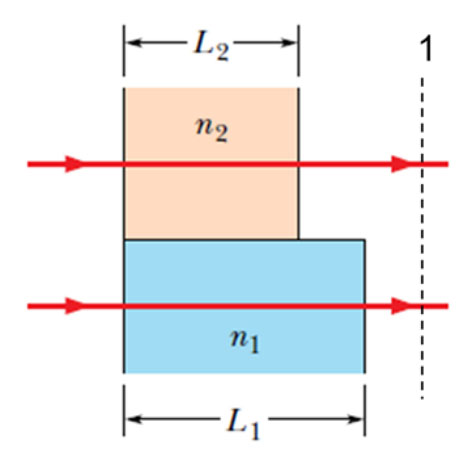
\includegraphics[scale = 0.2]{images/phasenverschiebung.jpg}
\end{center}
\begin{footnotesize}
	$k_0=\frac{2\pi}{\lambda_0}$\\
	$k_1=\frac{2\pi}{\lambda_0} n_1$\\
\end{footnotesize}
\\
\section{Reflexion und Transmission}
Energieerhaltung:
\[
	I_0=I_r+I_t \\ \Rightarrow \\ n_1 E_0^2= n_1 E_r^2+ n_2 E_t^2 \\ \\
\]
Definition:	
\[
	E_r=r\cdot E_0 \\ \Rightarrow \\ E_t=t\cdot E_0 \\
	\Rightarrow \\ 1+r=t\\
\]
Reflexions- und Transmissionskoeffizienten:
\[
	r= \frac{n_1-n_2}{n_1+n_2} \\ \Rightarrow \\ 
	t= \frac{2n_1}{n_1+n_2} 	\\ \\ \\
\]
\[
	I_r=|r|^2\cdot I_0  \\ \Rightarrow \\ 
	I_t=\frac{n_2}{n_1}|t|^2\cdot I_0 \\ \\
\]
\begin{itemize}
	\item $n_1 < n_2$: Reflektierte Welle erfährt einen Phasensprung von $\pi$, bzw. $\lambda/2$
	\item$n_1 > n_2$: Reflektierte Welle erfährt keinen Phasensprung \\
\end{itemize}
\
\section{Dünnfilm-Interferenz}
Bedingung reduzierte Reflexion:
\[
	d=m\frac{\lambda_0}{2n} \\ m=1,2,.. \\ \\
\]
Bedingung verstärkte Reflexion:
\[
	d=\frac{\lambda_0}{4n}+m\frac{\lambda_0}{2n} \\ m=0,1,..\\ \\
\]
\begin{center}
	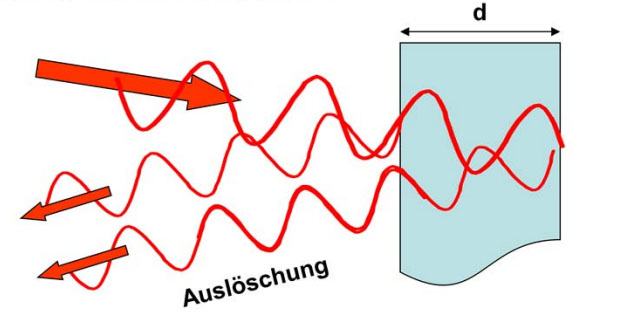
\includegraphics[scale = 0.2]{images/df_interferenz.jpg}
\end{center}
Die Reflexion beim Übergang zwischen zwei Medien mit Brechungsindizes $n_1$ und $n_2$ kann mit einer zusätzlichen Antireflexions-Dünnschicht reduziert werden. \\
$n_1< n_{AR}<n_2$ \\
\\
Schichtdicke $\frac{\lambda}{4 n_{AR}}$
\\
\\
Idealer Brechungsindex:
\[
	 n_{AR}^2=n_1\cdot n_2
\]
\\
\section{Fabry-Perot Interferometer}
Das Fabry-Perot Interferometer (Etalon) besteht aus zwei parallelen, reflektierenden Oberflächen in einem festen Abstand d mit einer Reflexion R<100. 
\\
\\
\textbf{ under construction}
\\
\section{Beugung am Spalt}
\[
	\sin\alpha_{min}=m\cdot \frac{\lambda}{D} \\
	\sin\alpha_{max}=(m+\frac{1}{2})\cdot \frac{\lambda}{D}	
\]
Für kleine Beugungswinkel gilt:
\[
	x_{min}=m\cdot\frac{\lambda}{D}L\\
	x_{max}=(m+\frac{1}{2})\cdot\frac{\lambda}{D}L\\ \\
	m=1,2,3...
\]
\begin{center}
	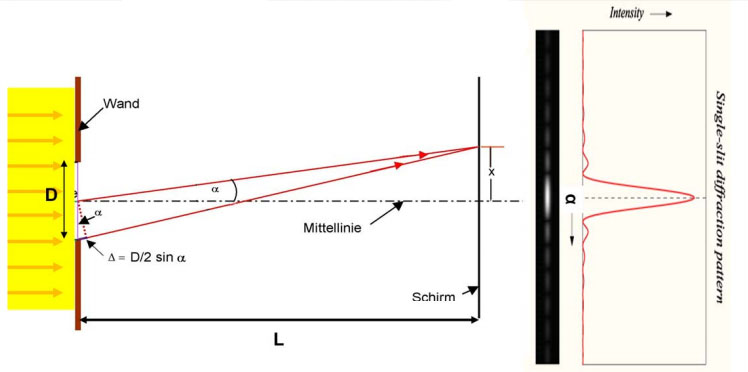
\includegraphics[scale = 0.3]{images/beugung_spalt.jpg}
\end{center}
Auflösungsvermögen Mikroskopie
\[
	\Delta l=1.22 \cdot \frac{f\cdot\lambda}{D}
\]
\begin{footnotesize}
	$f$:	Brennweite der Linse \\
	$D$:	Durchmesser der Linse\\
\end{footnotesize}
\\
\section{Beugung am Gitter}
Wenn Licht auf eine periodische Anordnung von Streukörpern trifft, können die Elementarwellen, die von den Streukörpern ausgehen in bestimmte Richtungen konstruktiv interferieren und ein Beugungsmuster generieren.
\[
	\sin \varphi_{max}=m\frac{\lambda}{a} \\
	x_{max}=m\frac{\lambda}{a}L \\
	m=1,2,...
\]
\begin{center}
	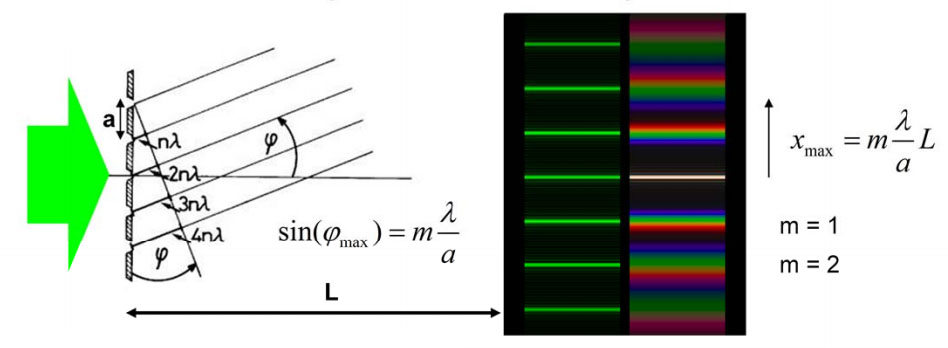
\includegraphics[scale = 0.25]{images/beugung_gitter.jpg}
\end{center}
\
\section{Polarisation}
\[
	E_t=E_0\cdot \cos\Delta\varphi \\
	I_t= I_0\cdot\cos^2(\Delta\varphi)
\]
Polarisationsgrad:
\[
	PG= \frac{P_{max}-P_{min}}{P_{max}+P_{min}}
\]
\\
\section{Transmission und Reflexion (Fresnell)}
\textbf{under construction}
\\
\section{Absorption}
Viele Materialien absorbieren einen Teil des Lichtes. Die Absorption hängt von der Wellenlänge ab und ist oft charakteristisch für ein Material.
\[
	I(d)=I_0\cdot 10^{-\alpha d} \\
	I(d)=I_0\cdot e^{-\alpha^* d} \\
	I(d)=I_0 \cdot 10^{\frac{-\alpha^` d}{10}}
\]
\[
	Chemiker \\ \\
	Physiker \\ \\ \\
	Optischer Ingenieur
\]
\begin{footnotesize}
	$\alpha^`$	in dB/m \\
\end{footnotesize}
\\
\section{Intensität Gauss Strahl}
Die Intensität quer zur Strahlrichtung hat die Form einer Gauss Kurve. Im Abstand r=W von der z-Achse fällt die Intensität auf 13.5\% $(e^-2)$ ab.
\[
	I(r,z)=\underbrace{I_0 \left(\frac{W_0}{W(z)}\right)^2}_{I(0,z)} 
	\cdot \underbrace{e^{-\frac{2r^2}{W(z)^2}}}_{Querschnittsprofil} 
\]
Strahlradius W(z):
\[
	W(z)=W_0\sqrt{1+\left( \frac{z}{z_0}\right) ^2}
\]
Mit $\pm z_0$ wird der Rayleigh Bereich (Tiefenschärfe) bezeichnet.
\[
	2z_0=\frac{2\pi W_0^2}{\lambda}
\]
Öffnungswinkel:
\[
	\theta_0 \approx \tan \theta_0 = \frac{\lambda}{\pi W_0} \\ \text{in rad } \\ \\
\]
\\
Gauss Strahlen:
\[
	W_{FWHM}(z)=1.18\cdot W(z) \\
	\theta_{FWHM} = 1.18 \cdot\theta_0 \\ \\
\]
\\
\section{Kollimierter Gauss Strahl}
Ein Strahl heisst kolimiert/gebündelt, wenn die Divergenz sehr klein ist. Man bezeichnet einen Strahl auch als kollimiert, wenn der Rayleigh Bereich des Strahls ungefähr gleich gross ist wie die relevante Propagationsdistanz der Anwendung.\\
\\
\[
	W_0^`=\frac{\lambda\cdot f}{\pi\cdot W_0} \geq
	 \frac{2\lambda\cdot f}{\pi\cdot D} 
	 \equiv \frac{2\lambda}{\pi} F_{N}
\]
\[
	\frac{W_0}{W_0^`}=	\frac{f_1}{f_2^`}
\]
\begin{center}
	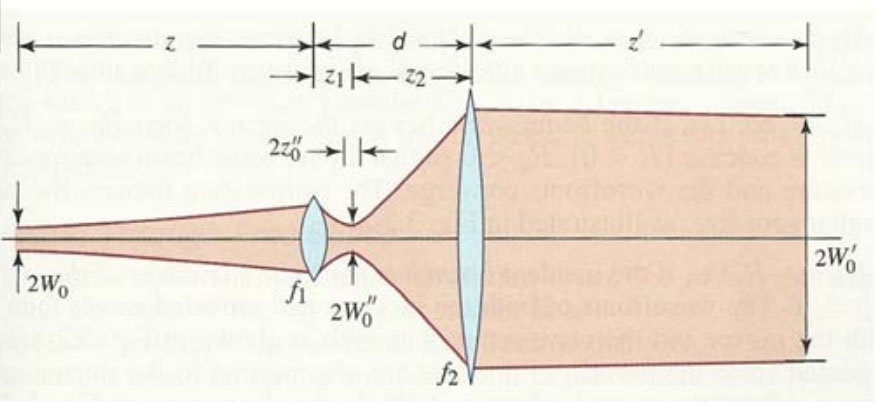
\includegraphics[scale = 0.25]{images/koll_gauss_strahl.jpg}
\end{center}
\
\\
\section{Wellenleiter}
\subsection{Metall-Wellenleiter}
Als einfachstes System eines Wellenleiters kann man zwei parallele metallene Oberflächen (Spiegel) nehmen.\\
\\
\textbf{Bedingung:} Wellenfronten von Reflexionen in die gleiche Richtung interferieren konstruktiv.\\
\\
\[
	\sin \theta_m= \frac{m \cdot \lambda}{2d}\\
	m=1,2,3,... \\ \\
\]
\\
Da der sinus maximal 1 sein kann, gibt es eine maximale Anzahl Moden:
\[
	M\leq\frac{2d}{\lambda}
\]
\[
	\lambda_c=2d
\]
wenn $\lambda> \lambda_c$ kann sich das Licht in dieser Art Wellenleiter nicht fortbewegen.\\
\
\[
	v_m=c\cdot \cos\theta_m=c\sqrt{1-m^2\cdot\frac{\lambda^2}{\lambda_c^2}}
\] 
\begin{center}
	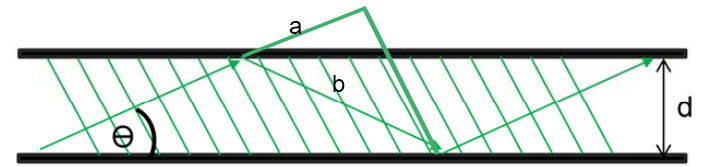
\includegraphics[scale = 0.3]{images/wellenleiter.jpg}
\end{center}
\
\\
\subsection{Dielektrische planare Wellenleiter}
Ein dielektrischer Wellenleiter besteht aus einem Kern und einem Mantel mit unterschiedlichen Brechungsindizes. Wenn \textbf{$n_1>n_2$} gibt es innerhalb eines Winkelbereichs Totalrefelxion und die Struktur funktioniert als Wellenleiter.\\
\\
\[
	\cos \bar{\theta_c}=\frac{n_2}{n_1}
\]
\[
	\tan (\pi \frac d\lambda \cdot\sin \theta_m-m\frac{\pi}{2})=
	\sqrt{\frac{\sin^2 \bar{\theta_c}}{\sin^2\theta_m}-1} \\
	m=1,2,3,.. 
\]
\\
Wie bei den metallischen gibt es zu jedem $\theta_m$ eine Mode, die propagieren. Die Anzahl der Moden ist durch $\theta_c$ beschränkt und beträgt: \\
\[
	M \dot{=} \frac{2d\cdot\sin \bar{\theta}_c}{\lambda} \\
	\dot{=}\frac{2d}{\lambda_0}\cdot NA\\ \\ \\ \\
	\dot{=}\rightarrow \text{nächst grössere ganze Zahl}
\] 
\[
	NA=\sqrt{n_1^2-n_2^2}=n_1\cdot \sin \bar{\theta_c}
\]
\begin{center}
	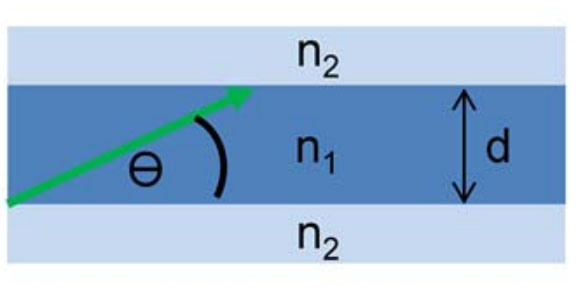
\includegraphics[scale = 0.2]{images/dielektrische_WL.jpg}
\end{center}
\
\begin{footnotesize}
	$NA:$	Numerische Aperatur \\
\end{footnotesize}
\
\\
\subsection{Modenprofil}
Die Eindrinktiefe nimmt mit der Modenzahl zu.\\
\[
	\delta_m=\frac{\lambda_0}{n_2 \cdot 2\pi}\left( \frac{\cos^2\theta_m}{\cos^2 \bar{\theta_c}} -1  \right)^{-\frac{1}{2}}
\]
\\
Im Unterschied zum metallenen Wellenleiter gibt es im dielektrischen immer eine Mode, selbst für sehr kleine $d$. Zu jeder Dicke gibt es jedoch einen cut-off Frequenz, unterhalb derer der Wellenleiter nur eine Mode zulässt.\\
\[
	f_c=\frac{c}{NA\cdot 2d}
\]
\\
Single mode wenn:
\[
	f<f_c \\
	\lambda > \lambda_c=2d\cdot NA
\]
\begin{center}
	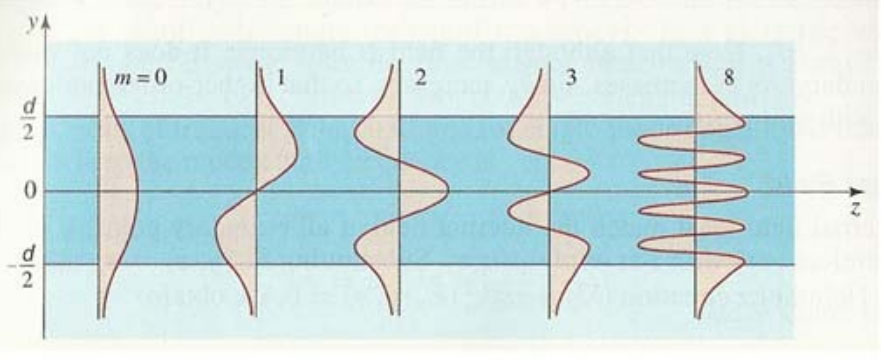
\includegraphics[scale = 0.2]{images/modenprofil.jpg}
\end{center}
\
\section{Optische Fasern}
\subsection{Singlemodefaser}
Optische Fasern bestehen aus einem Kern und einem Mantel mit unterschiedlichen Brechungsindizes. Es gibt Moden, deren Anzahl durch den Durchmesser des Kerns gegeben ist.\\
\\
Um einen geringen Verlust zu erlangen, muss der Strahldurchmesser dem Modeprofil entsprechen und die Strahldivergenz muss kleiner sein als:\\
\[
	\sin \theta_a=NA=\sqrt{n_1^2-n_2^2}
\]
Single Mode kann nur der Grundmode (m=0) propagieren für die Frequenzen unterhalb der cut-off Frequenz.
\[
	f_c=\frac{c}{NA\cdot 2.61a}
\]
\begin{footnotesize}
	$a:$	Kernradius \\
\end{footnotesize}
\\
\begin{center}
	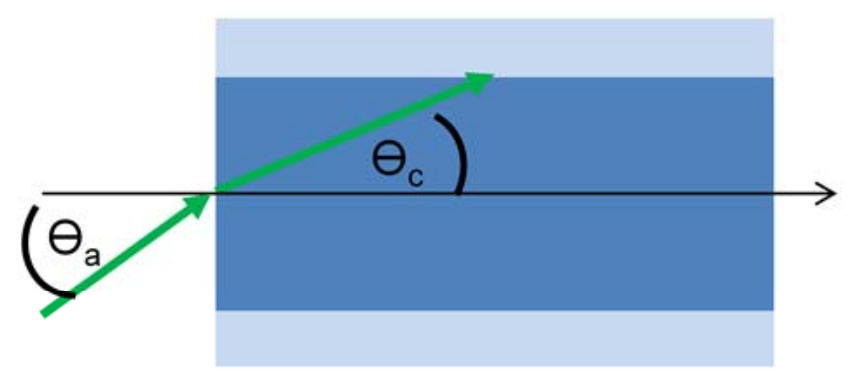
\includegraphics[scale = 0.15]{images/opt_faser.jpg}
\end{center}
\
\subsection{Multimodefaser}
Für Fasern mit grossem Kernradius a gilt:
\[
	M\approx \left( \frac{4a}{\lambda_0} \cdot NA \right)^2 
\]
\\
\section{Schwarzkörper-/Thermische Strahlung}
\textbf{Lord Rayleigh's} Berechnung beschreiben das Emissionsverhalten eines Schwarzkörpers für grosse Wellenlänge.\
\[
	K(\lambda,T)=2c \cdot k_B\cdot \frac{T}{\lambda^4}
\]
\textbf{Stefan-Boltzmann's} Formel beschreibt für das gesamte Emissionsvermögen des schwarzen Körper.\
\[
	R(T)=\sigma \cdot T^4 
	\\ \left[ R\right]  =\frac{W}{m^2} \\ \\
\]
\begin{footnotesize}
	$\sigma:$	$5.67040 \cdot 10^{-8} \frac{W}{m^2\cdot K^4}$ \\
\end{footnotesize}
\\
Die effektiv abgestrahlte Leistung eines realen Körpers mit Temperatur $T_1$ in einer Umgebung mit Temperatur $T_2$.\
\[
	\Delta P = \varepsilon \sigma A\cdot (T_1^4-T_2^4)
\]
\begin{footnotesize}
	$\varepsilon:$	Beschreibt die prozentuale Fläche unter der Kurve. \\
\end{footnotesize}
\\
\subsection{Wiensche Verschiebungsgesetz}
Verschiebungsgesetz von Wien für das Emissionsmaximum eines schwarzen Körpers als Funktion der Temperatur.\
\[
	\lambda_{max} \cdot T = 2.898 \cdot 10^{-3}m\cdot K
\]
\\
\section{Zeitliche Kohärenz}
Tie Kohärenzzeit $T_c$ ist gekoppelt mit der Breite des Spektrums $\Delta f$.\
\[
	\Delta f \approx \frac{1}{\pi\cdot \tau_c}
\]
%coding:utf-8

%----------------------------------------
%FOSAPHY, a LaTeX-Code for a summary of optics
%Copyright (C) 2014, Mario Felder, Michael Fallegger

%This program is free software; you can redistribute it and/or
%modify it under the terms of the GNU General Public License
%as published by the Free Software Foundation; either version 2
%of the License, or (at your option) any later version.

%This program is distributed in the hope that it will be useful,
%but WITHOUT ANY WARRANTY; without even the implied warranty of
%MERCHANTABILITY or FITNESS FOR A PARTICULAR PURPOSE.  See the
%GNU General Public License for more details.
%----------------------------------------

\chapter{Quanten Optik}
\section{Konstanten}
\[
\boxed{\begin{aligned}	
		&h = 6.62606872\cdot 10^{-34} J\cdot s \\
		&m_e = 9.1094\cdot 10^{-31}kg \\
		&k_B = 1.380658 \cdot 10^{-23} \frac{J}{K}\\
		&eV = 1.602176565 \cdot 10^{-19}J\\
		&\hbar = \frac{h}{2\pi}
	\end{aligned}}	\]
\\
\section{Grundformeln}
Umrechnung:
\[
	E_J = E_{eV} \cdot 1.602\cdot 10^{-19}
\]
\\
\section{Photon- das Lichtquantum}
Die maximale kinetische Energie nimmt linear mit der Frequenz des Lichts zu. Es wird kein Photostrom beobachtet für $f<f_0$.\
\[
	E=h\cdot f = \hbar \cdot \omega = \frac{h \cdot c}{\lambda}
\]
\begin{footnotesize}
	$h$:	Planck'sche Konstante = $6.62606872\cdot 10^{-34} J\cdot s$\\
\end{footnotesize}
\begin{center}
	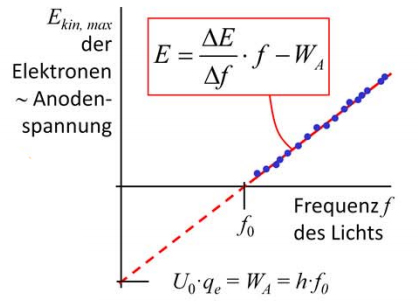
\includegraphics[scale = 0.3]{images/photon_energie.jpg}
\end{center}
\
\\
\section{Impuls des Photons - Compton Streuung}
Obwohl das Photon keine Ruhemasse besitzt, hat es trotzdem einen Impuls. Die Relativitätstheorie liefert für das Photon mit Wellenlänge $\lambda$ den Impuls $p$:\

\[
	p=\frac{E}{c}=\frac{h\cdot f}{c}= \frac{h}{\lambda}=m\cdot v \\ \text{pro Photon} \\ \\
\]
Energie- und Impulserhaltung liefern:
\[
	\Delta\lambda = \lambda^` -\lambda=\frac{h}{m_e\cdot c}\cdot \left( 1- \cos \phi  \right) = \lambda_c \cdot \left( 1- \cos \phi   \right) )
\]
Anzahl Photonen pro Sekunde:
\[
	n=\frac{P}{E}
\]
\begin{center}
	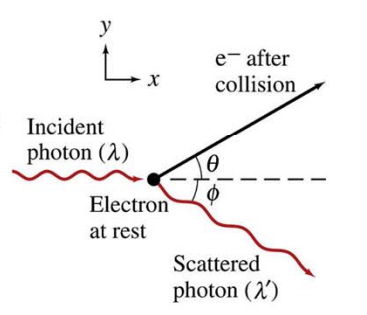
\includegraphics[scale = 0.3]{images/impuls_photon.jpg}
\end{center}
\
\section{Bremsstrahlung}
In einer Röntgenröhre werden Elektronen von einer geheizten  Kathode auf die Anode beschleunigt. Maximale Frequenz (kleinste Wellenlänge) kann ein Bremstrahlungs-Photon erreichen, wenn es die ganze kinetische Energie des Elektrons schluckt.\
\[
	q_e\cdot V_{AC} = h\cdot f_{max} = \frac{h\cdot c}{\lambda_{max}}=\frac{\Delta E}{h\cdot c}
\]
\\
\section{Energie}
In einem elektrischen Spannungsfeld, entspricht die Differenzspannung der Energie auf ein Elektron.\\
zB. 100V $\rightarrow$ 1 Elektron $\rightarrow$ 100eV
\[
	E= \frac{1}{2}\cdot m_0  v^2 = \frac{1}{2} \frac{p^2}{m_E}=\frac{p^2}{2m}
\]
\\
\section{Energieniveaus von Wasserstoff}
Balmer-Formel:
\[
	\frac{1}{\lambda}=R_y\cdot \left( \frac{1}{2^2} - \frac{1}{n^2}\right) 
\]
\begin{footnotesize}
	$R_y$=	$1.097\cdot 10^7 m^{-1}$\\
	$n$=	$3,4,5,...$ \\
\end{footnotesize}
\[
	E_n= -\frac{h\cdot c \cdot R_y}{n^2}
\]
\begin{footnotesize}
	$R_y$=	$1.097\cdot 10^7 m^{-1}$\\
	$n$=	$1,2,3,...$ \\
\end{footnotesize}
\begin{center}
	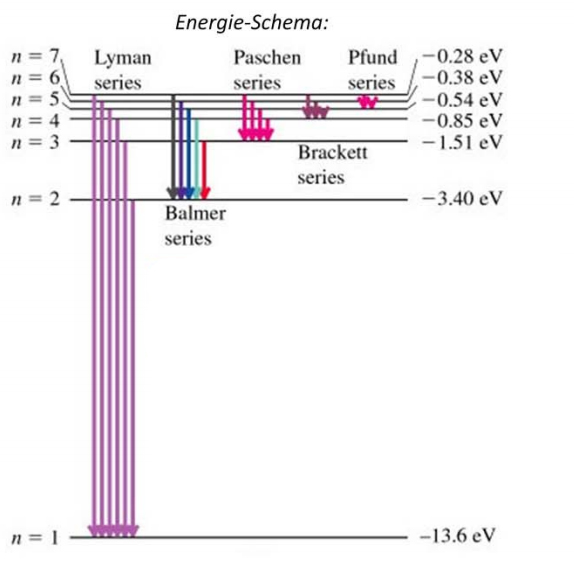
\includegraphics[scale = 0.25]{images/en_H.jpg}
\end{center}
\
\subsection{Bohr's Herleitung der Balmerformel}
Wasserstoff:
\[
	E_n= - \frac{1}{\varepsilon_0^2}\cdot\frac{m_e\cdot q_e^4}{8n^2\cdot h^2}
\]
Helium+:
\[
	E_n= - 
	\frac{1}{\varepsilon_0^2}\cdot\frac{m_e\cdot q_e^4}{2n^2\cdot h^2}
\]
\begin{center}
	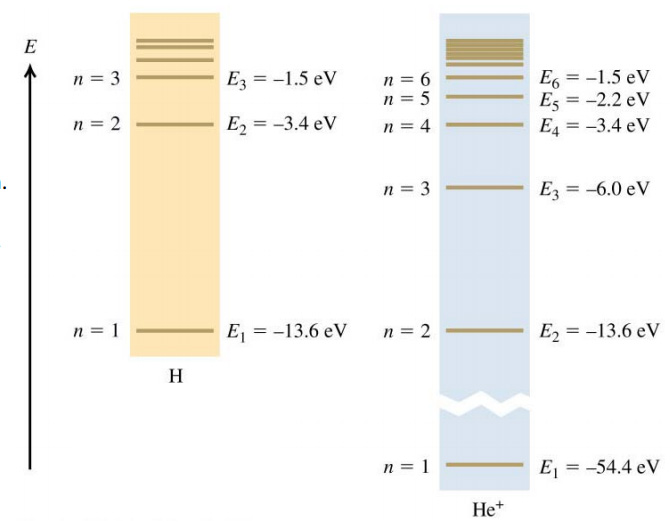
\includegraphics[scale = 0.25]{images/bhor_herleitung.jpg}
\end{center}
\
\\
\section{Energieschema}
\begin{center}
	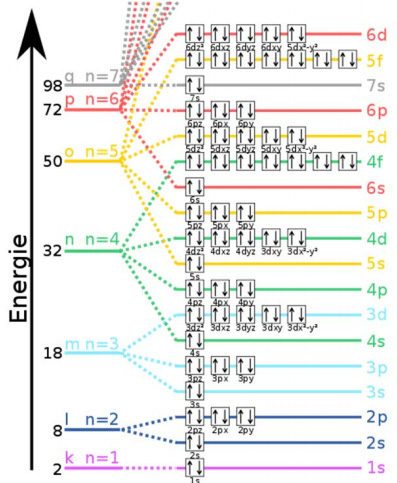
\includegraphics[scale = 0.3]{images/energieschema.jpg}
\end{center}
\
\\
\section{Spektrum des Natriumatoms}
\begin{center}
	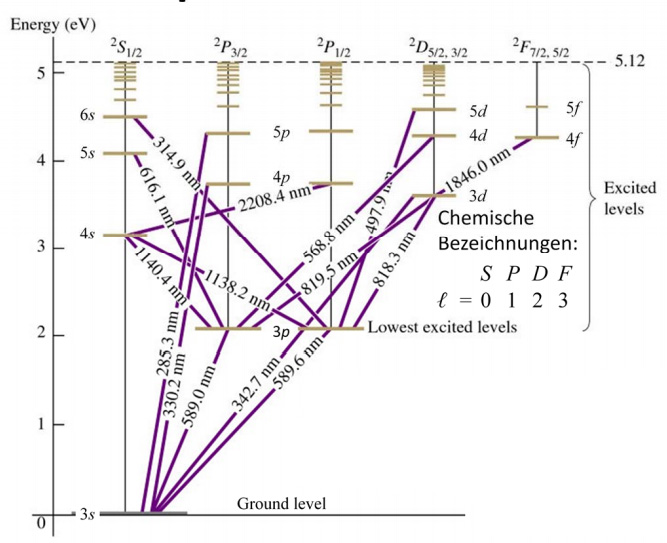
\includegraphics[scale = 0.3]{images/spektrum_na.jpg}
\end{center}
\
\\
\section{Niveaubesetzung und Besetzungsinversion}
Die Maxwell-Boltzmann-Verteilung der Geschwindigkeiten in einem Gas bei der Temperatur $T$ lautet:\
 $f(v,T)=C_1(T)\cdot v^2 e^{-\left( \frac{m_{kül} \ cdot v^2}{2k_B\cdot T} \right) }$\
 oder als Funktion der Energie: $f(E;T)=C_2(T)E\cdot e~{ \frac{E}{k_B\cdot T}}$.\
 \\
 Verhältnis der beiden Besetzungswahrscheinlichkeiten:
 \[
 	\frac{F(E_f,T)}{F(E_i,T)}=\frac{E_f}{E_i}\cdot e^{-\left( \frac{E_f-E_i}{k_B\cdot T}\right) }
 	\approx	
 	e^{-\left( \frac{E_{Gap}}{k_B\cdot T}\right) }
 \]
 \[
 	\frac{f_2}{f_1}=e^{-\left( \frac{1}{k_B\cdot T}  \right) }\left(  E_2-E_1 \right) 
 \]
 \begin{footnotesize}
 	$f$=	$e^{- \frac{E_1}{k_B \cdot T}}$\\
 \end{footnotesize}
 \
 \\
 \section{Quantenverschrkänkung = Superposition}
 $Hg_2$ Molekül:\\
 Wir sind gewohnt Teilsysteme als völlig unabhängig voneinander zu betrachten. Verschränkung bedeutet nun, dass die beiden Atome durch eine gemeinsame Wellenfunktion beschrieben werden. Es handelt sich bei der instanten Spinausrichtung des zweiten Atoms nicht um eine Nachrichtenübertragung im klassischen Sinn. Bei der Messung des ersten Atoms, wird die Ausrichtung des zweiten Atoms festgelegt.\
 \\
 \section{Polarisation und Photonen}
 Die Durchgangswahrscheinlichkeit $p$ der Photonen ist ene Funktion des Winkels $\theta$ (Gesetz von Malus):\
 \[
 	p(\theta)= \cos^2(\theta)
 \]
 \begin{center}
 	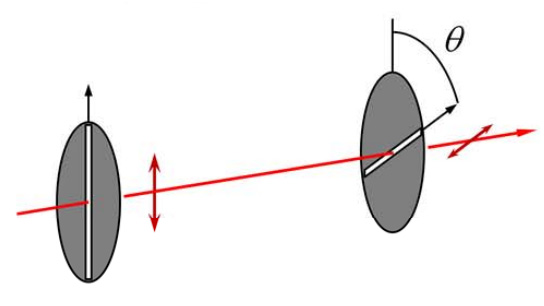
\includegraphics[scale = 0.3]{images/polarisation_photon.jpg}
 \end{center}
 Die Wahrscheinlichkeit, dass das $+z$ polarisierte Teilchen den zweiten Polarisator als $+s$ polarisiertes Teilchen passiert, beträgt:
 \[
 	p(\theta)= \cos^2(\frac{\theta}{2})
 \]
 \\
 \section{Verschränkung mit Photonen}
 Eine Quelle produziere verschränkte Photonenpaare. Die verschränkten Photonen fliegen in entgegengesetzte Richtungen und passieren Polfilter.\
 Die Wahrscheinlichkeit, dass beide Photonen die Filter passieren, ist:
 \[
 	p(\alpha,\beta)= \frac{1}{2} \cdot\cos^2(\alpha-\beta)
 \]
 \begin{center}
 	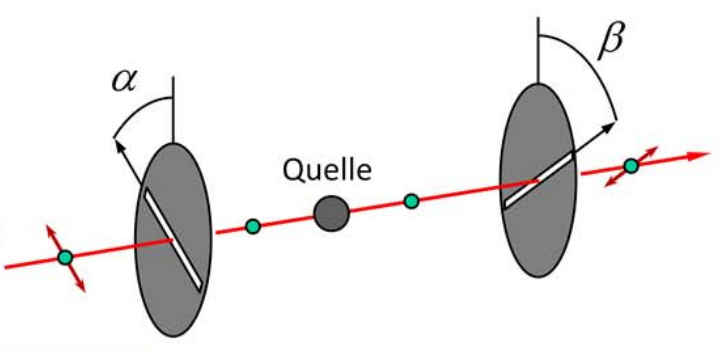
\includegraphics[scale = 0.2]{images/verschraenkung_photon.jpg}
 \end{center}
 \
 \\
 \section{Schrödingergleichung - Wellenfunktion}
 Schrödinger Gleichung:
 \[
 		i\hbar \dfrac{\partial\psi(x,t)}{\partial t}=
 		U(x)\cdot\psi(x,t)-\frac{\hbar^2}{2m}\frac{\partial^2\psi(x,t)}{\partial x^2}
 \]
 U ist eine (klassische) potentielle Energiefunktion, beispielweise die Coulombenergie eines Elektrons im Wasserstoffatom.\\
 \\
 \begin{footnotesize}
  	$\hbar$=	$\frac{h}{2\pi}$\\
  	$h$= $6.62606872\cdot 10^{-34}$\\
  \end{footnotesize}
  \
  \\
  Die Coulomb-Energie des Elektron um den Wasserstoffkern (=Proton):
  \[
  		U_{H-Atom}=-\frac{1}{4\pi\varepsilon_0}\cdot\frac{q_e^2}{r}
  \]
  Die potentielle Energie der Hooke'sche Feder (=harmonische Oszillator):
  \[
  		U_{harm. Oszillator}=\frac{1}{2}\cdot kx^2
  \]
  \\
  \section{Interferenz $\rightarrow$ Unschärferelation}
  Nach klassicher Interferenz gilt folgende Beziehung zwischen Winkelablenkung $\theta_1$, Wellenlänge $\lambda$ und Spaltöffnung $a$:\
  \[
  		\sin\theta_1\approx \theta = \frac{\lambda}{a}
  \]
   \begin{center}
   	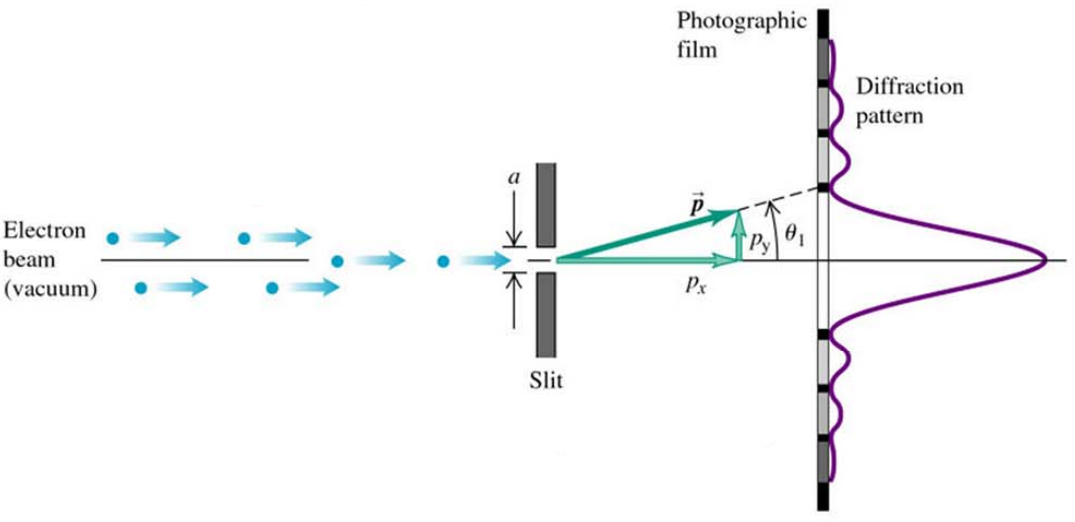
\includegraphics[scale = 0.2]{images/unschaerferelation.jpg}
   \end{center}
  Je kleiner die Wellenlänge $\lambda$, desto schärfer ist das Hauptmaximum. Oder je grösser der Spalt a, desto kleiner die Winkelbeugung.\\
  \\
  Die $y$-Beschränkung des Elektrons innerhalb $a$ erzeugt einen y-Querimpuls.
  \[
  		\underbrace{\Delta p_y=p_y}_{\text{Def. von $\Delta p_y$}}=
  		\underbrace{\tan\theta_1\cdot p_x \approx \theta_1\cdot p_x= \frac{\lambda}{a}\cdot p_x}_{\text{Beugung am Spalt}}=
  		\underbrace{\frac{\lambda}{a}\cdot\frac{h}{\lambda}}_{\text{De Broglie}}\equiv
  		\frac{\lambda}{\Delta y}\cdot\frac{h}{\lambda}
  		\rightarrow \Delta p_y\cdot\Delta y = h
  \]
\\
Heisenberg'sche Unschärferelation:
\[
	\Delta x \cdot \Delta p_x \geq \frac{h}{\pi}= \frac{\hbar}{2}	
\]
ebenso:
\[
	\Delta y \cdot \Delta p_y \geq \frac{\hbar}{2}	\\ \Delta z \cdot \Delta p_z \geq \frac{\hbar}{2} \\ \\
\]
\
\\
\section{Tunneleffekt}
Ein klassisches Teilchen mit Energie $E<U_0$ kommt nicht über diese Potentialbarriere. Es wird an der Wand reflektiert. Die Schrödingergleichung erlaubt aber Lösungen $\psi(x,t)$ wie in der Figur. Ein Teilchen, das ursprünglich links der Hürde ist, hat eine Wahrscheinlichkeit $T$, durch das Hindernis zu tunneln.\
\\
\[
	T=G\cdot e^{-2\kappa\cdot L}\ll 1
\]
\[
	G=16\cdot \frac{E}{U_0}\cdot \left( 1-\frac{E}{U_0}\right) 
\]
\[
	\kappa = \frac{\sqrt{2m\cdot\left( U_0-E  \right) }}{\hbar}
\]
Aufenthaltszeit:
\[
	\Delta t \cdot \Delta E < \hbar
\]
\
\\


\end{document}

